\chapter{Work Done}\label{C:workdone}

\section{Overview}
There were three main goals before the preliminary report. Firstly, create a framework to trace a tests spectrum. This not only included writing the aspect but also ability to pipeline the analyse algorithms. Secondly, find suitable bench marks meeting a certain criteria. Lastly, research and implement several different analysis methods.

\section{Creating the Framework}

The first goal of the project was to create a framework to trace tests and allow for different analysis methods to be added and changed with ease. The first question that arose was, what was the best way to execute every test? Since AspectJ with load time weaving was determined to be the best method to trace, a build automation tool would be best suited. Using a build automation tool will remove a lot of redundancy during the analysis and execution of the tests. Its allows for a script to be written that will be run each time from a single command line argument, rather than having to repeat a long winded command line argument every time \todo{Feels broken?}. The two main choices were Ant and Maven. After doing research, Ant appeared to give more control over the execution of JUnit tests \cite{antjunit} \cite{mavenjunit}. It gave the ability to create a single new java virtual machine (JVM) before the tests were executed which would be used solely for the test suite. Since a static class to hold the trace data was used, the data needed to be held in memory until all the tests had run, which meant the tests had to be run with the same JVM. But the JVM had to be recreated as AspectJ load-time weaving requires its own class loader to be used through the command line java option. 

The ability to allow for a user defined pipeline is important in limiting the amount of hard coding. Ant uses it’s own JUnit runner class to execute the tests. This means that parameters would be difficult to input without executing the Ant file through another main method in order to create the pipelines. Doing this would be create messy and unwanted code. Therefore a properties file was the other viable approach which would be loaded in during the static method construction. The purpose of this properties file was to not only a change to the settings of a run, such as the results file name, the type of service it should use but also allowing for a ‘pipeline’ approach to be used. This pipeline will be used for the analysis where the pipeline can specify the type of analysis and its setting, shown in figure \ref{fig:pipeline}. The main pattern used to limit the amount of hard code when parsing the file was factory patterns. \todo{Show class diagram of a pipeline?}

\begin{figure}[h]
\caption{Pipeline}
\label{fig:pipeline}
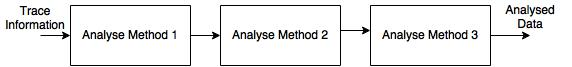
\includegraphics[width=\textwidth]{Pipeline.jpg}
\end{figure}


\section{Finding Benchmarks}

The second goal was to find suitable benchmarks; this was harder than it seemed. The benchmarks had to meet a criteria where they were java based, had large number of test cases (100 +) and were open source. Although there were over 10 potential benchmarks, the ability to use them depended on their build process. If they used Maven, it was difficult to create a jar that contained the tests and often meant that the amount of effort needed to get a working benchmark was higher than the benefit from it. This eliminated several potential benchmarks and left the Ant and gradle built projects. 

The current set of benchmarks is as follows:

\begin{itemize}
\item Whiley
\item Java Compiler Kit
\item Jasm
\item Spring - Core
\item Metric-x - Core
\item Ant
\end{itemize}


Using Ant as a benchmark created an unique situation. Since Ant is used to run the JUnit tests, I have made my aspect ignore Ant calls so that when Ant is executing the tests it does not get traced. However, if I ignore Ant calls then the Ant benchmark can not be traced. This meant that I had to not use Ant to run itself but manually execute it. This was deemed worth the effort due to Ant’s current stature within the development community. 

\section{Implementing Analysis Methods}

The third goal was to use the data to analyse and determine the tests that are closely related. The first analysis stage that I decided to use was Levenshtein distance metric. This metric is the minimum number of single-character edits, in our case method calls where edits are either insertions, deletions or substitutions. This method created some challenges. Firstly, the time to compare every test with every test becomes exponential. So as the analysis became more computationally heavy, the time to analyse the data increased. Secondly, due to there being thousands of tests and each test containing tens of thousands of method calls, memory management became crucial. 

My first approach was to resolve both issues by using a bloom filter approach. A bloom filter is a test where you determine whether an element is a member of a set or not, returning either "possibly in set" or "definitely not in set" \cite{bloomfilterwiki}. In this case, it was used to determine whether the set of method calls for two tests were similar or not. The similarity and analysis type are set within the property file. Looking at the set of method calls, rather than a list meant the number of comparisons decreased. Using a 99 percent similarity for the 'bloom filter' on the wyc package of Whiley, this meant the next analysis stage had 232 comparisons, rather than 187922. This approach was used under the hypothesis that the following is true.

$A, B, C, D \neq A, D, E, F, G$

$A, B, C, D \approx A, B, C, D, E$

That the first case the two tests would be not be redundant test’s due to having a high difference in method calls. However, there is a chance that the second test may be the same so it implies more computational heavy analysis should be done on it, such as using a list of method calls. This means that when using a list of method calls, the amount of data held in memory will be reduced as the number of tests will be decreased from the initial stage.

Although this made the analysing stage faster, it did not have any effect on the testing time. Each time that an analysis was to be run, the tests needed to be run at the same time. The approach used to get around this was to save the test data to disk. Such that the properties file can be set to save the data to disk, and when the data wants to be used without analysis, a main method is called. However, analysing was still taking a substantial amount of time. \todo{Provide figures?}

To increase the performance of analysis, I decided to implement a concurrent method. The framework was implemented such that it was able to be done relatively easy. When testing the execution on a test environment, the results between concurrent and non concurrent gave the same result. However, on a benchmark the result was different. This required thinking about whether the test environment was too limited. David Pearce suggested a larger test environment be created. Through doing this it allowed the errors to be found and in turn the concurrent execution was fixed. The concurrent execution lead to an increase of up to 2 times faster analysis; however it required more memory. This was because in the non current mode, the spectrum of a test could be decoded and analysed. After analysis, the object would be nulled allowing for the garbage collector to free the memory. However, during concurrent execution, the decoded objects were only nulled after a full pipeline execution as another thread may be using that object. \todo{Not to sure if this is explained very well}

The next analysis implementation was the total difference. This method discarded the order of the methods for a test. Instead sorted them alphabetically and for every difference between the pairs, it added the 1 to the difference. This worked well in conjunction with the bloom filter approach, as it was a fast analysis pipeline while still returning high accuracy results. \todo{Should I explain what high accuracy is ?}

The next idea implemented was to take into account for the ‘calling context tree’. This means that for each method call, the data contains a separate node for each call stack that the method was called with \cite{callingcontext}. What this involves in java terms is using the stack trace of the method and storing the depth specified within the properties file. It is therefore more difficult for a test to be similar to another as the calling tree of a method call is used.

Finally, the last implemented method was weighting. The idea behind it was that there are some methods that will be contained within the majority of tests spectrum and occur frequently in the spectrum. These methods will often be low level, such that every test will execute them. Therefore giving less information about the level of redundancy than lower frequency method calls. So the idea in weighting is to increase the 'importance' of lower frequency method calls by discarding the top 20\% method calls.

\section{Results}
\todo{Should I compare the current analysis methods ? ie. Show more results such as the number of redundant tests each method gives ?}
The result that will be shown will be from the Whiley benchmark using the Levenshtein distance metric. From looking at the graphical representation \ref{fig:similiartests}, it shows the tests that are matching for Byte\_Valid\_5 test.

\begin{figure}[h]
\caption{GUI showing similar test cases}
\label{fig:similiartests}
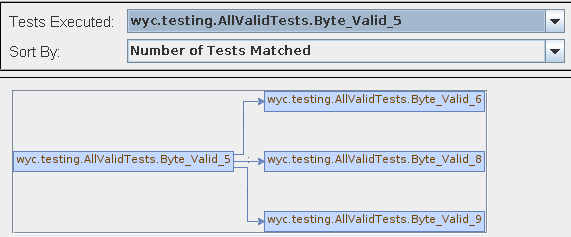
\includegraphics[width=\textwidth]{model24.png}
\end{figure}

This requires us to conduct further examination of the test and as such the tests are from the Whiley Compiler tests, so looking at the Whiley files would give us insight into how closely related these two tests are. Comparing Byte\_Valid\_5 and Byte\_Valid\_8 in figures \ref{fig:byte8} and \ref{fig:byte5} respectively. It shows that the difference between the tests is the range of j and two additional addition statements. The decision whether these two tests are redundant is up to a developer. But there is a possibility that they could be separated or merged to create a single test case.

\begin{figure}[h]
\caption{Byte\_Valid\_8}
\begin{lstlisting}
public method main(System.Console sys) -> void:
    for i in constants:
        for j in 0 .. 8:
            sys.out.print(Any.toString(i) ++ " << ")
            sys.out.print("1+" ++ Any.toString(j) ++ " = ")
            sys.out.println(Any.toString(i << (1 + j)))
\end{lstlisting}
\label{fig:byte8}
\end{figure}

\begin{figure}[h]
\caption{Byte\_Valid\_5}
\begin{lstlisting}
public method main(System.Console sys) -> void:
    for i in constants:
        for j in 0 .. 9:
            sys.out.print(Any.toString(i) ++ " << ")
            sys.out.print(Any.toString(j) ++ " = ")
            sys.out.println(Any.toString(i << j))
\end{lstlisting}
\label{fig:byte5}
\end{figure}



